\documentclass[15pt]{article}
\usepackage[utf8]{inputenc}
\usepackage[pdftex]{graphicx}     
\usepackage{amssymb}
\usepackage{ragged2e}
\title{CS3523 assignment 3}
\author{cs20btech11005 }
\date{February 2022}

\begin{document}

\maketitle

\begin{itemize}
\item The file basic.h contains some structures and classes that are required for EDF and RMS scheduling algorithms. It also contains a common part of scheduling algorithm of EDF and RMS scheduling.
\item Both EDF and RMS scheduling have different rules but the structure of their algorithms is similar.\\
The algorithms take input from inp-params.txt and store in an array called $input_data()$.\\
Then a scheduling algorithm which follows the rules of RMS and EDF schdeules the processes into an array called $sched_set()$.
\item The output is generated to "RMS-Log.txt" and "RMS-stats.txt" incase of RMS scheduling and "EDF-Log.txt" and "EDF-stats.txt" incase of EDF scheduling.
\item Some problems that arised while writing algo's are
\begin{itemize}
\item To calculate the waiting time initially I had to write a while loop that adds 1 to each process that is not running but this cause the time taken to run increase significantly and processes that have completed running also had their waiting time incresed.\\
There was a quick fix by having data of which process compled but it was not efficient.\\
So I added a variable to the $input_data$ class and made changes so that the deadline time is increased after each process finishes execution.
\item Another problem was to include the context-switch time, for this I added a variable to the stimulation algorigth in basic.h that holds the value of context switch time. and also the problem where the default unit of time wasn't precise enough so I had to increase the precision by multiplying the time values by 100.
\item While writing preemption if the running queue is empty but all processes haven't completed processing because they haven't joined yet, the program was showing preemption eventhough it was not for this also I just added some code and eliminated it.
\item Another similar issue was with calculating the number of missed deadlines. The problem was that a process that is not currently running can also miss deadline. So I had to add a for loop and a variable to prevent counting twice.
\end{itemize}
\end{itemize}
\begin{figure}[ht]
    \centering
    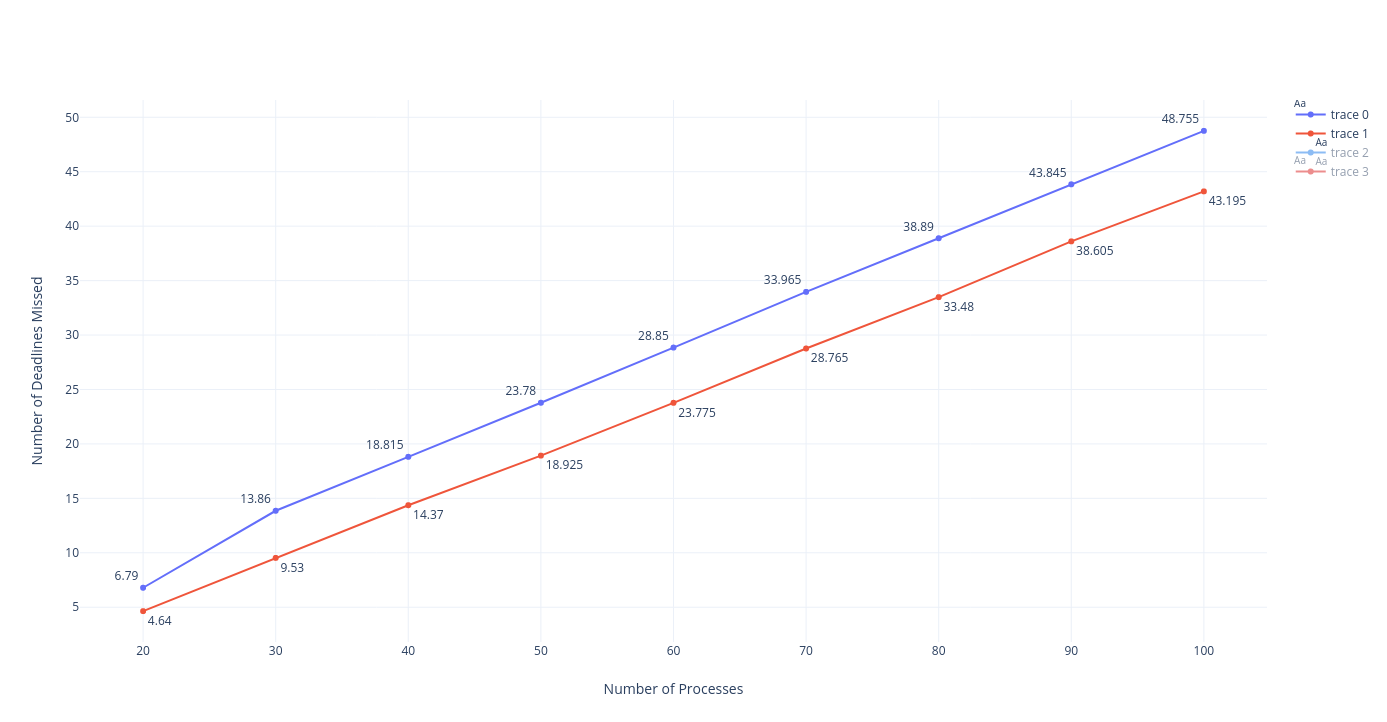
\includegraphics[width=1.25\textwidth]{1os2-assgn3.png}
    \caption{NO.OF Deadlines missed vs NO.OF Processes}
    \label{fig:Deadlines missed}
\end{figure} 

\begin{figure}[ht]
    \centering
    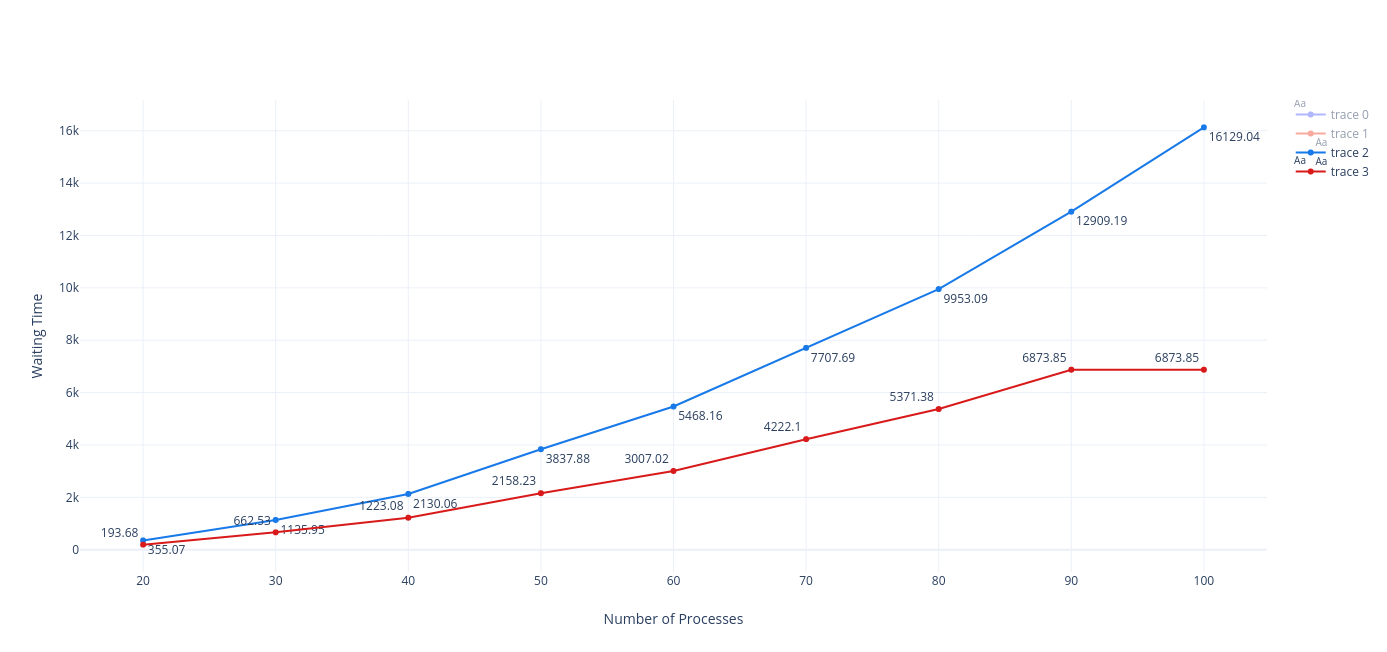
\includegraphics[width=1.25\textwidth]{os2-assgn3.png}
    \caption{Waiting Time vs NO.OF Processes}
    \label{fig:waiting time}
\end{figure}
The red lines/dots represent EDF scheduling.\\
The blue lines/points represent RMS scheduling.
\end{document}